% Drawing 138/07-8 -- folder 138, batch 07, archive page 126 (PDF page 127).
% Transcription: un polygone dont le bord est doublé d'une courbe ondulée, avec un éventail de triangles issus d'un sommet intérieur ; à droite, plusieurs disques et ellipses avec un rayon marqué $z$, un cône.
% Kind: polygon with wavy boundary and fan; discs, ellipses, cone. Method 2 (schematic redraw from the facsimile). Status: ok.
% Notes: Left: a polygon of eight sides drawn as his separate strokes (the top side, the right side in three pieces, the middle one thick, the lower right side, the bottom side, which stops short of the lower left vertex, the lower left side and the left side), with the short tick under the dot at the upper left vertex; a closed wavy curve round it; a fan of five rays from an inner vertex to the five vertices on the right side, the short stroke from the middle of the fan to the right side, and the sixth, faint stroke outside the fan, from the right side near its middle down to the lower right corner. Right column: an ellipse with a thick ray from a point near its centre to the right end and a dotted line from the left end to that point, and below it the second pencil pass of its lower half; a small tilted closed curve in ink (upper arc) and pencil (lower arc and a short faint piece at the upper left) with a point at each end; a disc with a ray from a point on its left boundary (with a short stroke up-right from that point), solid to the middle and dotted to the right, marked z; a cone (its left side straight, its right side nearly vertical) over an ellipse; a flat triangle: two sides from the apex (the left one faint), a stroke down from the apex, the base, and a separate short stroke to its right. Second pass 2026-11-14 (issue 147, Claude Opus 5.5): all of it redrawn stroke by stroke from grid overlays at 18 to 38 px per unit (the earlier redraw had the polygon as one closed path through its vertices, the sixth stroke and the tick left out, the pencil ellipse as a full second ellipse, the disc ray solid to the edge, and the flat triangle about 2 units off). The rasterised redraw laid over the crop: every stroke on its ink to within about half a unit. Not covered by this mark: the segment [0, 1] and the pentagon with marked midpoints in the middle (07-9), the bottom of the rhombus at the top right (07-7), the formulas « f(z) in [0,1] », « f(z) - 1/2 », « S = 0, 1, infinity » (text), and the long faint pencil stroke at the lower left, which crosses the page. Nothing is struck. Not compiled (no TeX engine in the session).
% Coordinates: 1 unit = 1 mm = 1/100 of the crop width (bbox in page fractions: [0.147, 0.508, 0.853, 0.716]).
% Redrawn by Claude (claude-opus-5-5), issue #73, 2026-11-09; not checked by a human; not compiled (no TeX in the session).
% Checked by Claude (claude-opus-5-5) 2026-11-14 (issue #147, second pass): strokes redrawn from the 300 dpi colour render of the 250 ppi scan, coordinates read on a grid overlay and checked by overlaying the rasterised redraw; not compiled (no TeX in the session). Not checked by a human. Status: ok.
% Rights: reproduces part of the work -- behind RENDER_TRANSCRIPTS, never published by itself.
\documentclass[tikz,border=3pt]{standalone}
\usepackage{amsmath,amssymb}
\usetikzlibrary{patterns,arrows.meta}
\tikzset{pencil/.style={black!45}, struck/.style={black!35}, mark/.style={circle,draw,inner sep=1.3pt}, pt/.style={circle,fill,inner sep=0.9pt}, opt/.style={circle,draw,fill=white,inner sep=1.1pt}}
\begin{document}
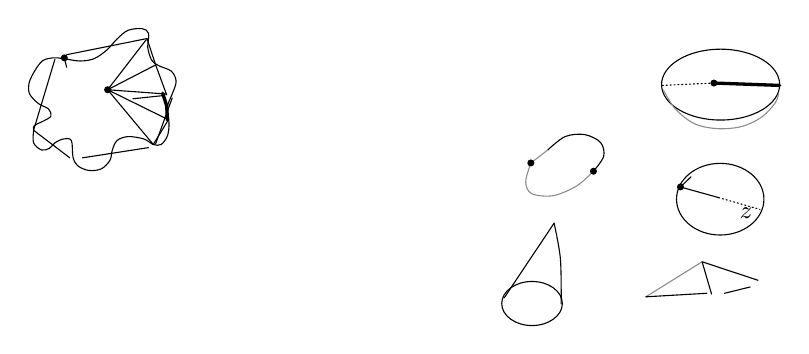
\begin{tikzpicture}[x=1mm,y=1mm,line cap=round,line join=round,font=\scriptsize]
\draw (7.2,-6.1) -- (17.4,-4.05);
\draw (17.4,-4.05) -- (18.5,-7.4) -- (19.9,-11.2);
\draw[very thick] (19.4,-11) -- (19.9,-12.6) -- (20,-14.4);
\draw (20.1,-14.4) -- (18.2,-17.5);
\draw (9.2,-19.2) -- (17.6,-17.9);
\draw (3,-15.7) -- (7.6,-19.2);
\draw (5.7,-6.7) -- (3,-15.7);
\draw (6.9,-6.5) -- (7.2,-7.7);
\draw (20.6,-11.6) -- (18.5,-17.4);
\draw (12.4,-10.55) -- (17.3,-4.2);
\draw (12.4,-10.55) -- (18.5,-7.4);
\draw (12.4,-10.55) -- (19.9,-11.1);
\draw (12.4,-10.55) -- (20,-14.3);
\draw (12.4,-10.55) -- (18.2,-17.5);
\draw (15.6,-11.7) -- (19.4,-11.3);
\node[pt] at (12.4,-10.55) {};
\node[pt] at (6.9,-6.5) {};
\draw plot[smooth cycle, tension=0.55] coordinates {(6.8,-6.6) (8.9,-6.9) (10.7,-6.6) (12.3,-5.5) (13.6,-4.1) (15,-3) (16.8,-2.8) (17.6,-3.4) (17.5,-5.2) (18,-6.8) (18.9,-7.5) (20.5,-8.2) (21.1,-9.5) (20.6,-11.1) (20,-12.7) (20.2,-14.8) (20,-16.4) (19.2,-17.5) (18.2,-17.5) (17,-16.8) (15,-16.5) (13.6,-17) (13,-18.2) (12.7,-19.5) (11.6,-20.6) (10,-20.8) (8.6,-20.2) (8,-19.1) (7.8,-17) (6.8,-16.8) (5.7,-17.3) (5,-18) (4,-18.2) (3,-17.3) (3,-15.7) (3.1,-15.1) (4.3,-14.5) (5.2,-13.9) (4.9,-13) (3.6,-12.3) (2.5,-11.1) (2.4,-9.8) (3,-8.4) (4.1,-6.9) (5.5,-6.5)};
\draw (90.25,-9.9) ellipse[x radius=7.5, y radius=4.5];
\draw[pencil] plot[smooth, tension=0.55] coordinates {(83,-10.6) (84.5,-13) (87,-14.9) (90,-15.5) (93,-15.2) (95.5,-14) (97.2,-12.2) (97.6,-11)};
\draw[very thick] (89.4,-9.7) -- (97.75,-10);
\draw[densely dotted] (82.85,-10) -- (89.4,-9.7);
\node[pt] at (89.4,-9.7) {};
\draw plot[smooth, tension=0.55] coordinates {(68.3,-18.2) (70.5,-16.5) (73,-16.25) (75,-17.25) (75.4,-19) (74.1,-20.9)};
\draw[pencil] plot[smooth, tension=0.55] coordinates {(74.1,-20.9) (72,-22.75) (69,-24) (66.25,-23.75) (65.5,-22.25) (66.15,-19.85)};
\draw[pencil] (66.15,-19.85) -- (68.3,-18.2);
\node[pt] at (66.15,-19.85) {};
\node[pt] at (74.1,-20.9) {};
\draw (90.2,-24.45) ellipse[x radius=5.55, y radius=4.55];
\draw (85.15,-22.9) -- (90,-24.25);
\draw[densely dotted] (90,-24.25) -- (95.25,-25.75);
\draw (85.15,-22.9) -- (86.5,-21.6);
\node[pt] at (85.15,-22.9) {};
\node[inner sep=1pt] at (93.5,-26.2) {\small $z$};
\draw (66.3,-37.7) ellipse[x radius=3.85, y radius=2.8];
\draw (69.1,-27.5) -- (62.75,-37);
\draw plot[smooth, tension=0.55] coordinates {(69.1,-27.5) (69.9,-32) (70,-37.75)};
\draw (87.9,-32.4) -- (95,-34.75);
\draw[pencil] (87.9,-32.4) -- (80.75,-36.85);
\draw (87.9,-32.4) -- (89.1,-36.5);
\draw (80.75,-36.85) -- (88.5,-36.4);
\draw (90.75,-36.4) -- (94,-35.6);
\end{tikzpicture}
\end{document}
